\chapter{Machine Description}

The Cooper Union for the Advancement of Science and Art has never, in its history, owned its own Tube Notcher. For this reason, the Cooper Union Machine Co sought to design and build one for the institution. This machine will not just meet the same capabilities of Tube Notchers currently on the market but will surpass them in its design capabilities and will do so at a fraction of the cost.

\section{Overview}

Cooper Union Machine Co.'s Tube Notcher is a variable speed, 4 degree of freedom, variable radius notching machine for hollow tubing. Designed for The Cooper Union's student machine shop, the machine has a small footprint, can be operated by an amateur machinist, and is low cost. To meet its design requirements, the machine was broken into 4 main subsystems; the structure, the driveline, the fixturing mechanism, and the electrical system. 

\begin{figure}[H]
    \centering
    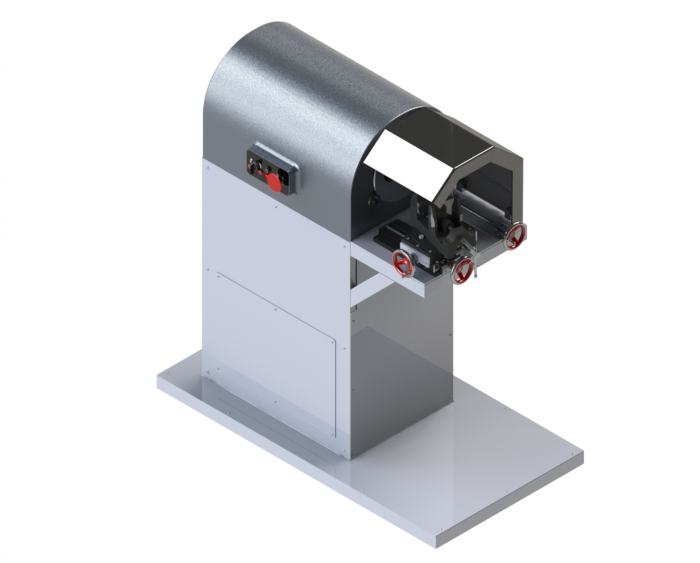
\includegraphics[width=0.7\textwidth]{./fall-report pictures/Chapter2-MachineDescription/FullSystemRender}
    \caption{Full SolidWorks rendering of Cooper Machine Co's Tube Notcher}
    \label{fig:FullSystemRender}
\end{figure}


\newpage

\section{Description of subsystems}

As mentioned in the previous section, the four subsystems of the tube notcher are the structure, the driveline, the fixturing mechanism, and the electrical system. The structure is composed of 3 parts; the frame, the shell, and the headstock. Its purpose is to support the weight of the machine itself, to withstand all forces generated while the machine is in use, and to facilitate the placement of the other subsystems for a user-friendly experience. The driveline is the largest of the 4 subsytems. It consists of the variator, eccentric, and spindle. Its purpose is to change the speed of the machine for use with different materials, allow for cuts of variable radius, and to house the end mill and collet during use. The fixturing mechanism is used to hold the workpiece in place and accommodate a variety of workpiece configurations relative to the cutting edge. Additionally, the fixturing mechanism must withstand the direct cutting forces during machining. Finally, the electrical system considers the electrical components of the system including the motors, switches, and controls for the machine. It also implements many of the safety mechanisms of the design itself. 

\newpage
\subsection{Structural}

\begin{figure}[H]
    \centering
    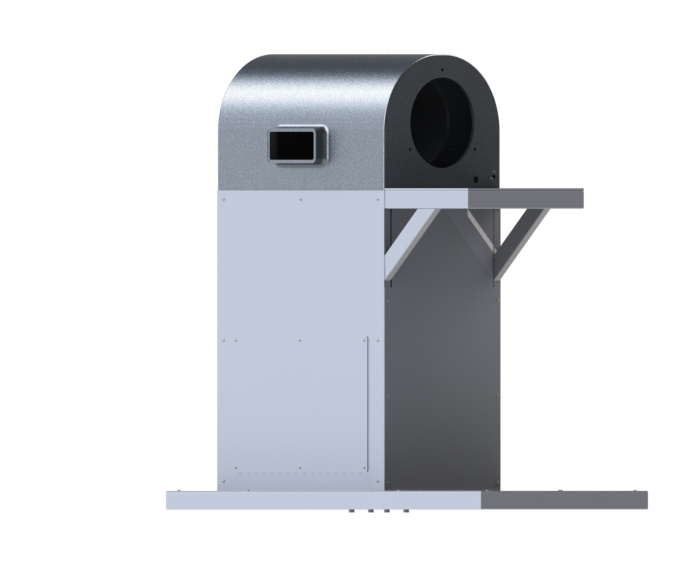
\includegraphics[width=0.8\textwidth]{./fall-report pictures/Chapter2-MachineDescription/Structural}
    \caption{SolidWorks rendering of the frame and shell design}
    \label{fig:Frame and Shell}
\end{figure}

The Notchmatic's structure provides the strength of the machine and is the central body to which the other three  subsystems are mounted to. The most critical part of the structure is the need to withstand the various static and dynamic loads that it experiences. This not only allows the Notchmatic to function properly while maintaining the precision of the cut but also keeps the user of the Notchmatic safe from potential failure due to excessive or unexpected loading conditions. The frame portion of the machine is designed to handle these loads. The shell is expected to experience some vibrations, at most, during machine operation. The main purpose of these components is to house all of the driveline parts, keep parts clear from metal shavings and other debris, keep the user away from dangerous components, and allow access to critical items for maintenance.  Maintenance is critical to ensure a long life-span and consistent accuracy of the machine. The variator motor needs to be regularly lubricated, electronics must be regularly accessed, belts have to be checked for wear, and OSHA requirements need to be satisfied. 

\begin{figure}[H]
    \centering
    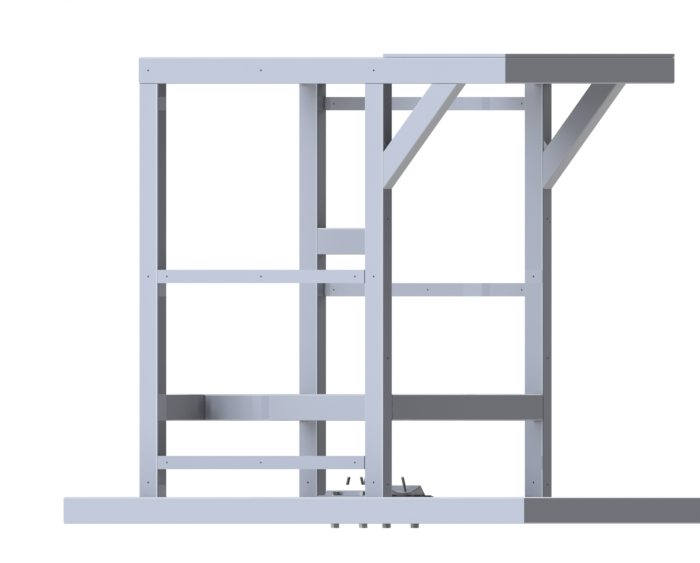
\includegraphics[width=0.6\textwidth]{./fall-report pictures/Chapter2-MachineDescription/Frame}
    \caption{SolidWorks rendering of the Frame}
    \label{fig:Frame}
\end{figure}

The frame is largely constructed of hollow steel rectangular tubing and a single steel sheets spanning the length of the machine, as shown above.  The frame of the machine provides the majority of the support and has mounting holes for the variator motor, variator pulley, spindle motor, and control box. A custom  motor mount was created for the main spindle motor using a 0.25in steel plate. This was tested for natural frequency, and is not in the range affected by operation speed of machine; thus avoiding harmonic vibrations. Further damping prevents fastening from coming undone and makes overall installation more secure. For these dampers, rubber sheet was chosen over sandwich dampers to decrease cost and size. The mount has 6 mounting holes and sits at the base of the design. A rendering of the motor mount is shown below.

\begin{figure}[H]
    \centering
    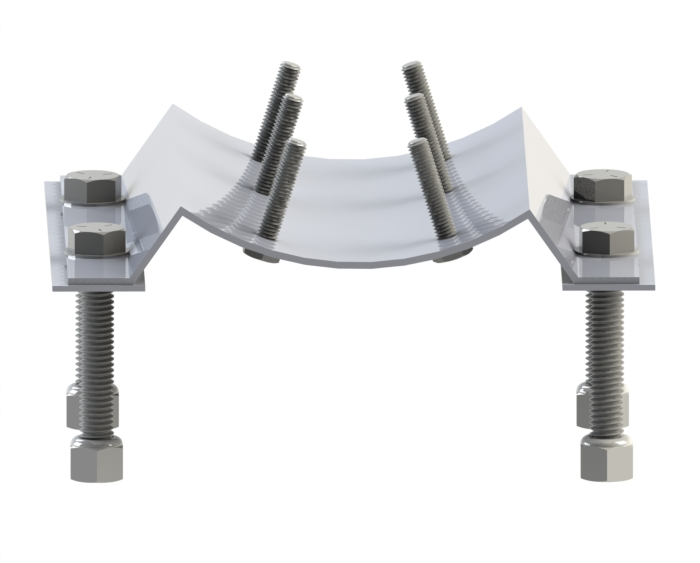
\includegraphics[width=0.6\textwidth]{./fall-report pictures/Chapter2-MachineDescription/MotorMount}
    \caption{SolidWorks rendering of the Motor Mount}
    \label{fig:Motor Mount}
\end{figure}

The final component of the frame is the steel bed. The bed is made from a single 0.25in steel plate. At the cutting end, it includes a latticed rib pattern. This greatly increases bed strength and, for that reason, is a common technique used in industry. This bears the heaviest loads during machine operation. On the other end, a diagonal cross support beam supports the bed. The bed will be constructed separately and then fit into the overall frame; allowing for easier installation of the fixturing mechanism and headstock. The figure below shows the underside of the steel bed to show the support members that add strength to the structure. The right end is where the cutting for the machine takes place. As described earlier, this part of the frame experiences the highest loads. Another reason to have an overdesigned bed is to reduce the deflection of the bed itself. Reducing the deflection increases the precision of the machine and can allow workpieces with higher tolerences to be machined. 

\begin{figure}[H]
    \centering
    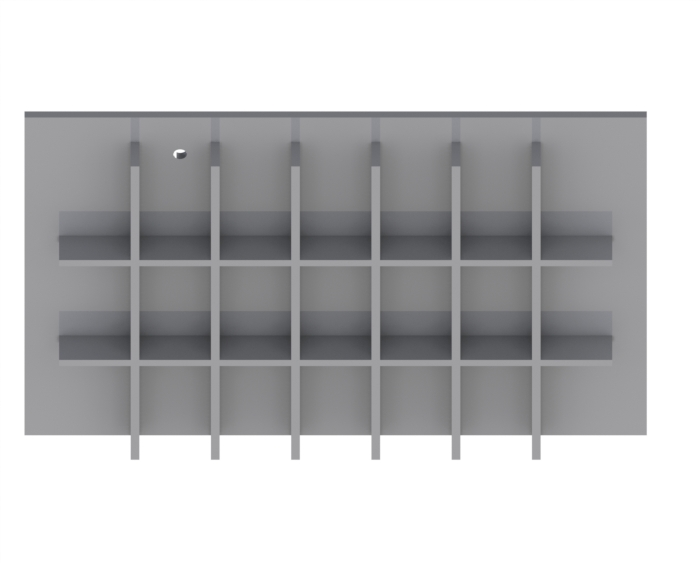
\includegraphics[width=0.6\textwidth]{./fall-report pictures/Chapter2-MachineDescription/Bed}
    \caption{SolidWorks rendering of the Bed}
    \label{fig:Bed}
\end{figure}

\newpage

\begin{figure}[H]
    \centering
    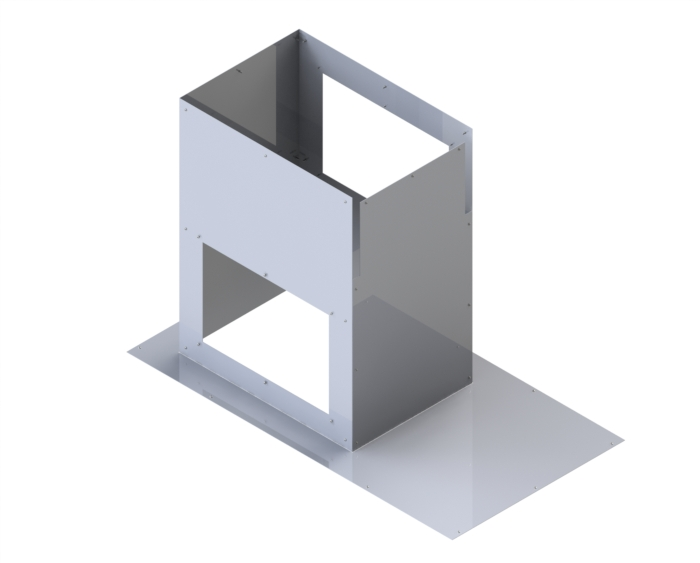
\includegraphics[width=0.6\textwidth]{./fall-report pictures/Chapter2-MachineDescription/Shell}
    \caption{SolidWorks rendering of the Shell}
    \label{fig:Shell}
\end{figure}

The shell of the Notchmatic, seen above, is the next biggest section of the structure of the machine. Initially, the shell was made from 18 gage aluminum sheets, but has since been replaced with 18 gage steel sheets. This material change reduces the surface damage of the machine resulting in a longer machine life. The shell is made of 5 separate steel sheets to simplify the fabrication of the machine. Welding copious amounts of thin steel sheets together would have been difficult, and aluminum would not have been plausible. The benefits of using the steel sheets for cost, strength, a machinability made the switch from to aluminum to steel a clear and obvious decision. The steel sheets are attached to the frame (one on each side of the machine and one at the base). The base plate completes the machine's aesthetics instead of leaving exposed frame.
 
There is a hole in the middle of the base sheet frame, and no two sheets should be in contact in order to avoid possible vibrations issues. Additionally, the base frame prevents the machine from tipping over. The three side faces, excluding the side plate under bed, may be manufactured as a continuous sheet of steel. The minimum radius that can be bent from 18 gage sheet steel is smaller than .12 (the corner radius of the frame members), thus allowing the shell to be fastened securely to the frame. This is dependent on the machine shop's ability to bend three feet of 18 gage steel. Currently, the 5 sheet set up are fastened to the frame using bolts, as shown below. It's important to note that these bolts are offset from the corners to avoid tapping into welds. Also, internal-tooth locking washers are being used in lieu of split lock washers. While both would mitigate vibration-caused loosening on fasteners, the second provides a more finished look. Wheels will later be included to give mobility to an otherwise very heavy machine. They will be supported by welded-in. Bushings provide extra strength at these points.


\begin{figure}[H]
    \centering
    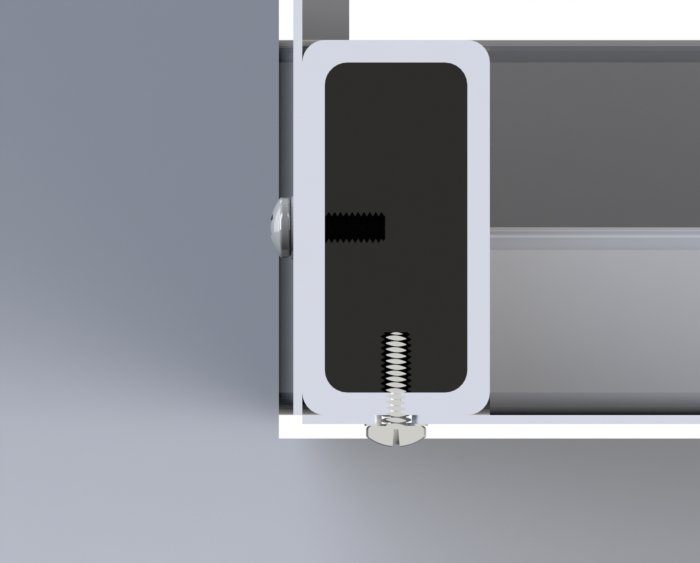
\includegraphics[width=0.6\textwidth]{./fall-report pictures/Chapter2-MachineDescription/ShellBolt}
    \caption{SolidWorks rendering of the Shell Fasteners}
    \label{fig:ShellBolts}
\end{figure}

\newpage
%Headstock
The headstock of the Notchmatic has the same pupose as the shell in addition to supporting the carrier plate support bearings and control panel. The Headstock will be cast from approximately 57 lbs of 6061 aluminum. The flat faces on the inside of the casting support the carrier plate while the remaining portion protects the driveline from debris. The headstock also has holes to facilitate other components. On the front there is  a mounting boss for the control panel and on the side of the cutting edge there is a hole for the eccentric drive handwheel shaft and for the safety shield shaft. Finally, there are holes in the base of the headstock so that it mounts to the steel bed of the frame. The figure below is the headstock casting alone used in the Notchmatic's design.

\begin{figure}[H]
    \centering
    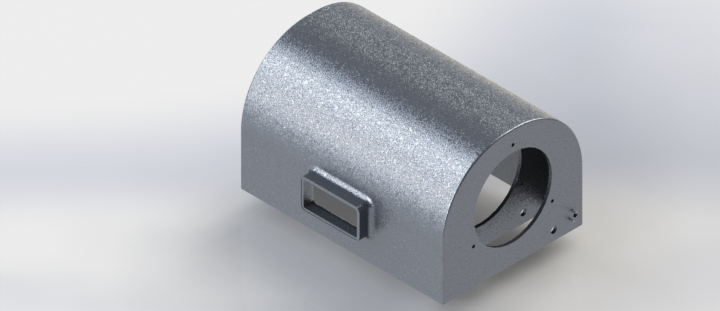
\includegraphics[width=0.6\textwidth]{./fall-report pictures/Chapter2-MachineDescription/Headstock}
    \caption{SolidWorks rendering of the Headstock Design}
    \label{fig:Headstock}
\end{figure}

Detailed drawings of the fasteners used, machined parts, and assemblies can be found in Chapter 4.

\newpage

\subsection{Driveline}

\begin{figure}[H]
    \centering
    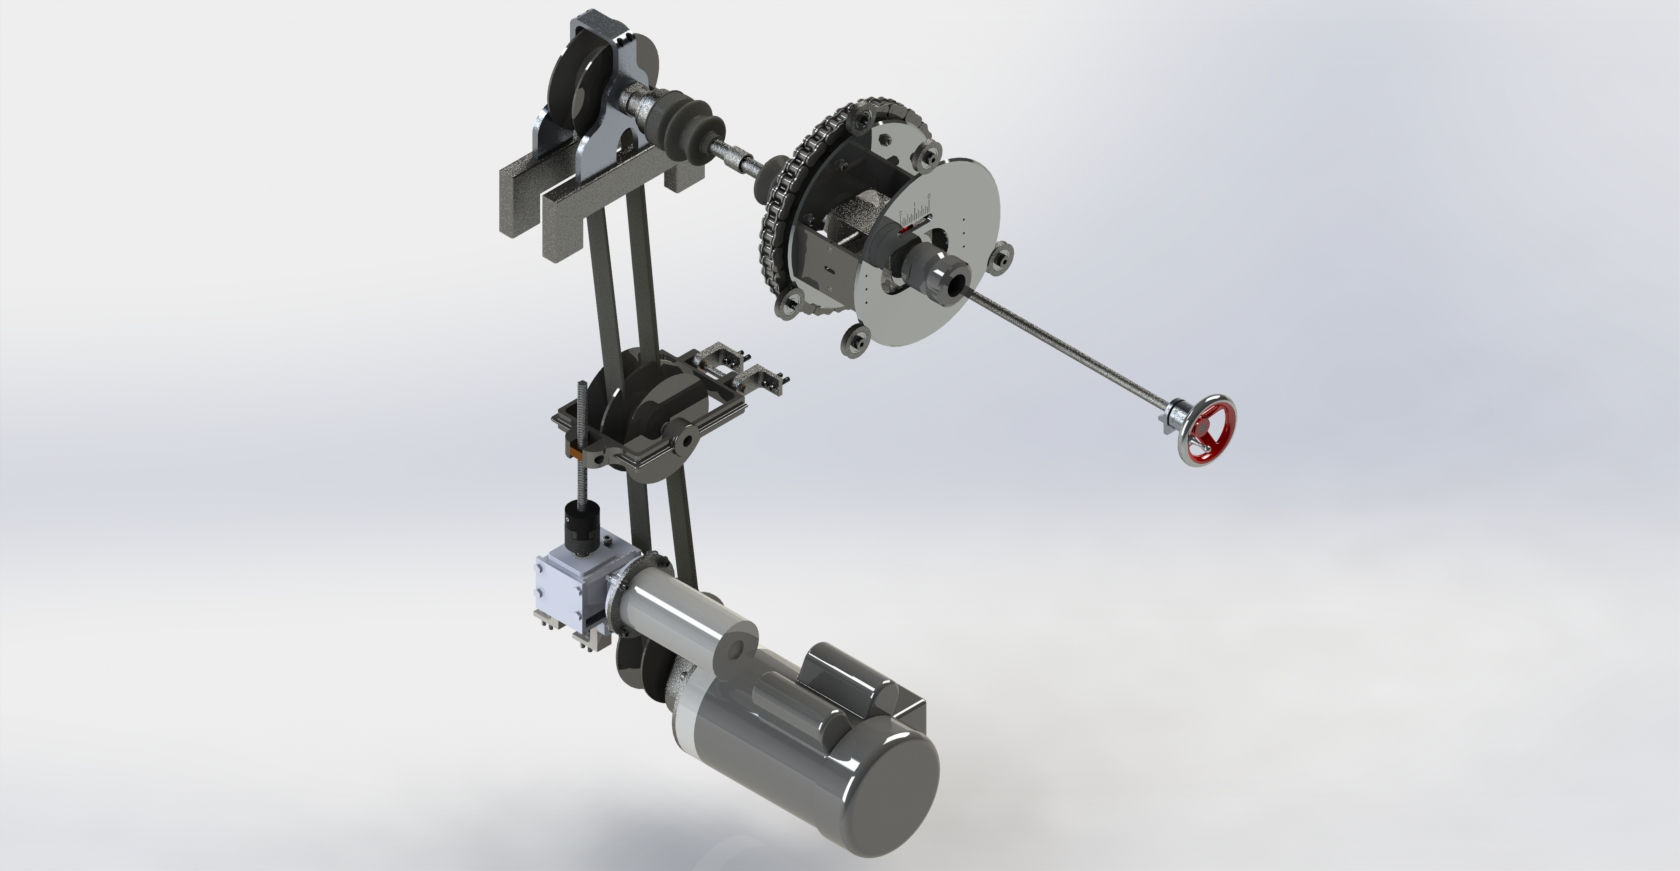
\includegraphics[width=0.8\textwidth]{./fall-report pictures/Chapter2-MachineDescription/Driveline}
    \caption{SolidWorks rendering of the Driveline}
    \label{fig:Driveline}
\end{figure}


The Notchmatic’s driveline subsystem transmits power from the electric motor to the end mill. The subsystem is further broken into three discrete parts: the spindle gearbox, the variator assembly, and the headstock driveshaft. The electric motor chosen to run the Notchmatic is a 1.5hp 110/220 VAC split phase squirrel cage motor. Due to the build constraints, this motor operates at approximately 1725 RPM. While this upper RPM bound is good for steels, and cast irons, for metals like aluminum, brass, and copper, much higher spindle speeds are recommended.  Initial conservative calculations suggested that the Notchmatic would need at most 2/3hp for the heaviest possible cut the machine would be able to perform. Therefore the decision was made to step up gear up the motor’s output speed 2.5:1.  To accomplish this, a pair of helical gears rated for 2hp was selected from Boston Gear’s extensive gear catalogs. Helical gears were chosen for their smoother running capabilities as well as their smaller form factor. 

\begin{figure}[H]
    \centering
    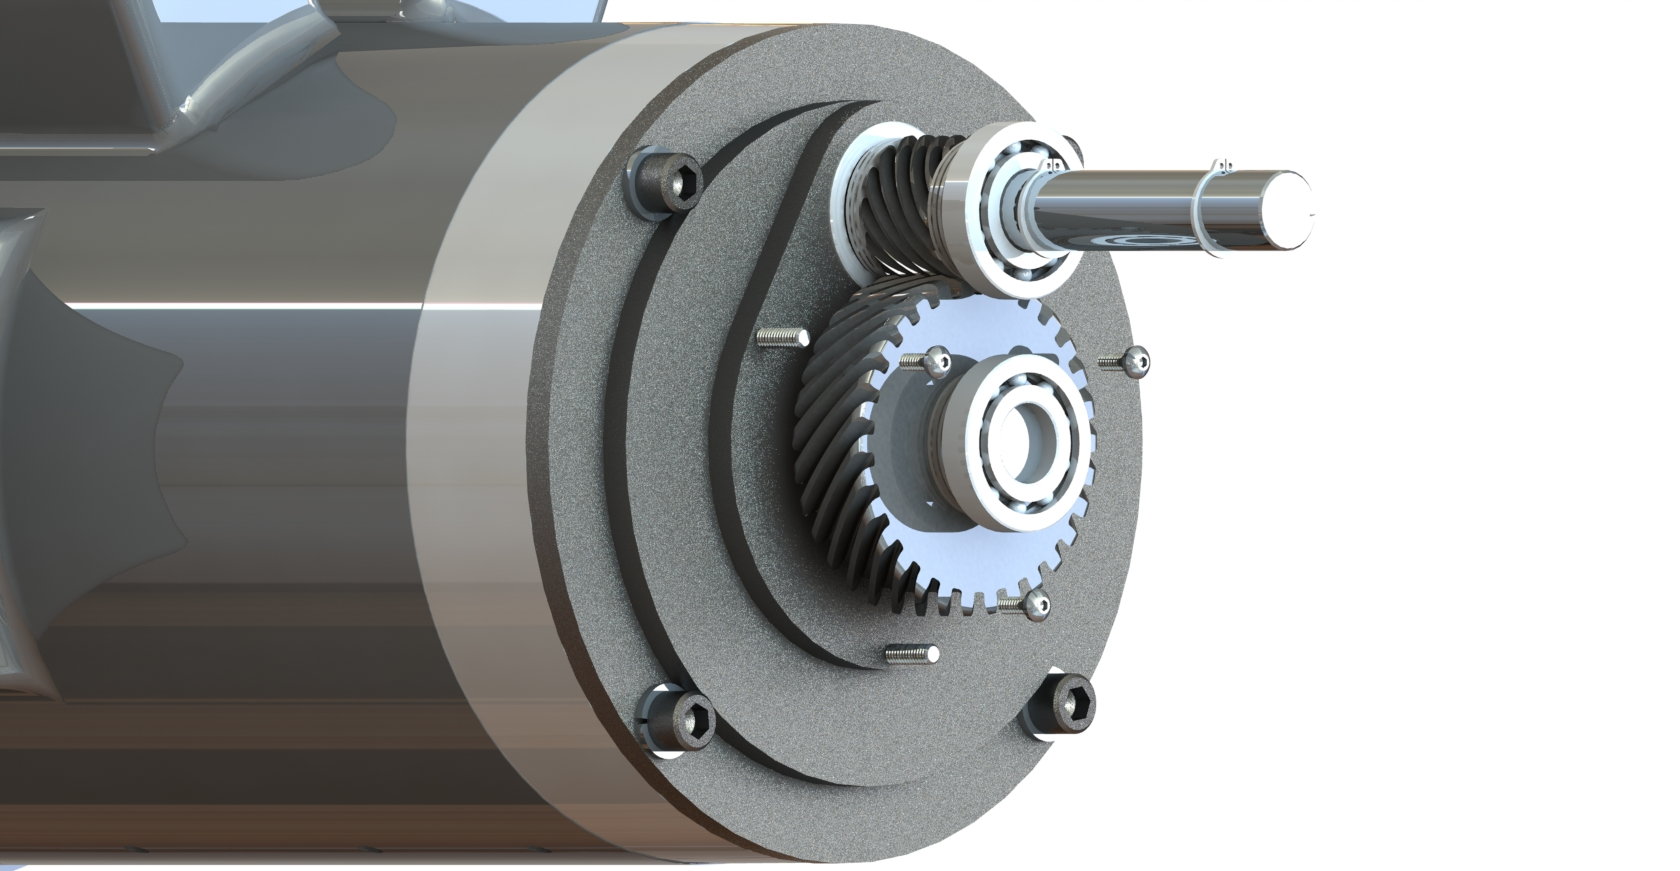
\includegraphics[width=0.6\textwidth]{./fall-report pictures/Chapter2-MachineDescription/GIA}
    \caption{SolidWorks rendering of the Gearbox Internal Assembly}
    \label{fig:GIA}
\end{figure}

One of the inherent downsides to helical gears however was their need for thrust compensating bearings. While this complicated the gearbox assembly, the relative cost savings and smaller form factor were deemed more important. The output shaft of the spindle gearbox runs to the bottom-end variable speed pulley. While this pulley has the same 16° slope as the variator pulleys, the bottom-end variable speed pulley has a fixed thickness. This ensures that the belt rides at one level of the pulley. 

\begin{figure}[H]
    \centering
    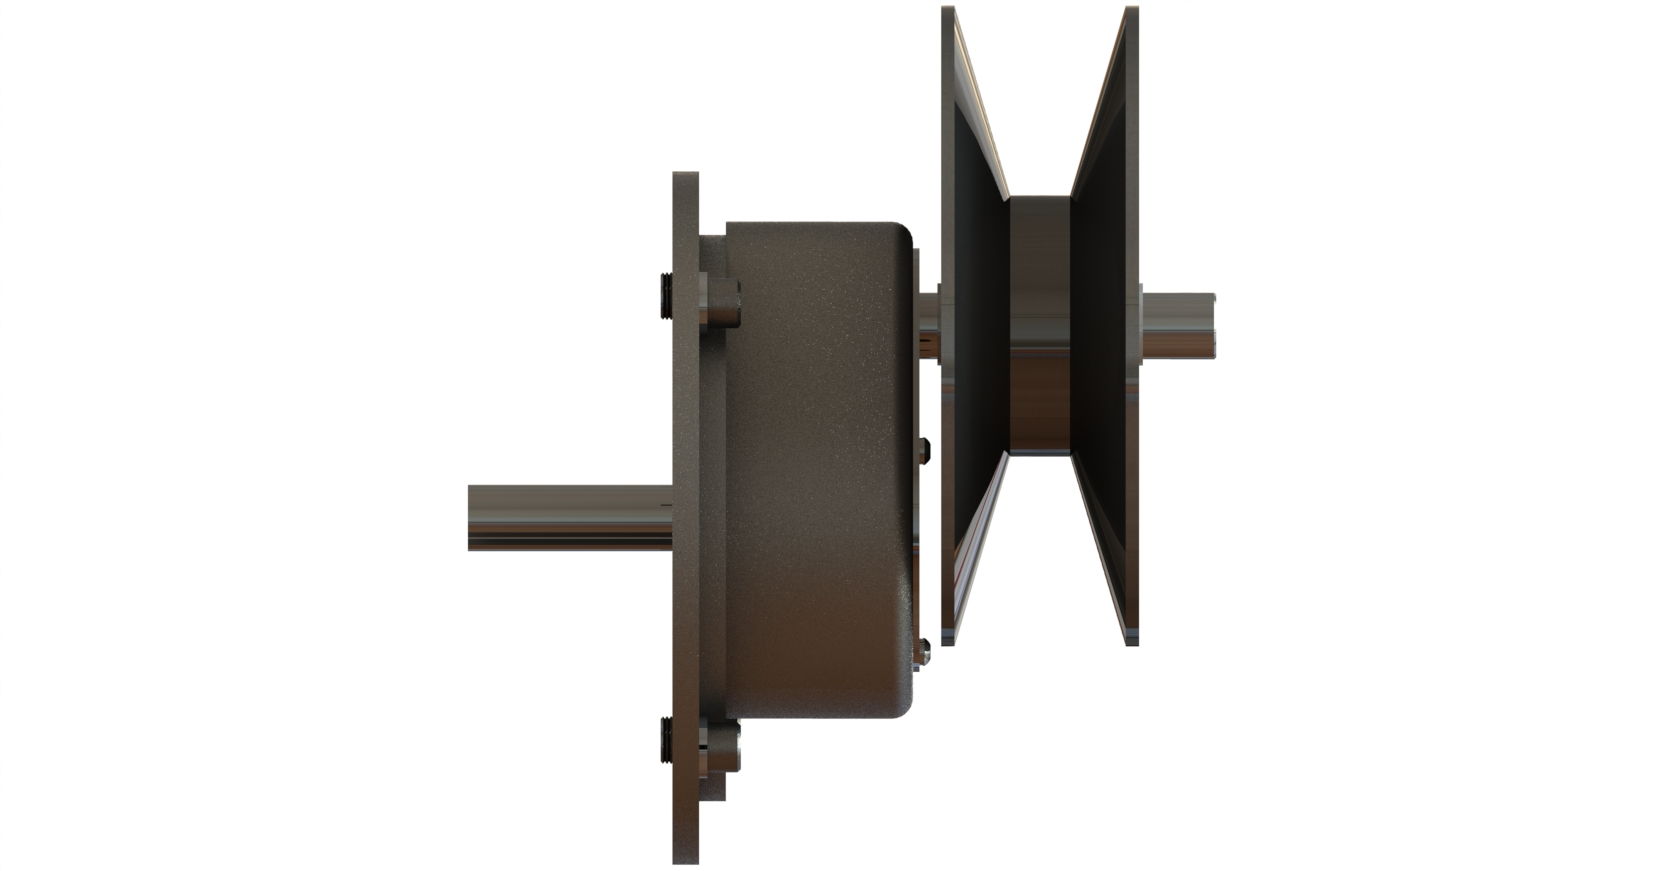
\includegraphics[width=0.6\textwidth]{./fall-report pictures/Chapter2-MachineDescription/GPA}
    \caption{SolidWorks rendering of the Gearbox and Pulley Assembly}
    \label{fig:GPA}
\end{figure}

The lower variable speed belt that runs from the bottom-end variable speed pulley to the variator assembly.  This assembly serves to continuously modulate the spindle speed of the Notchmatic over a range from 100 rpm to 4300 rpm. This wide speed range is obtained achieved by the linking of the angular position of the variator frame with the position of the pulley core. Based on the position of the frame, belt tension from either the upper or lower belt will continuously adjust the location of the core. The core location has a direct relationship with the effective pulley radii of the upper and lower pulleys.

\begin{figure}[H]
    \centering
    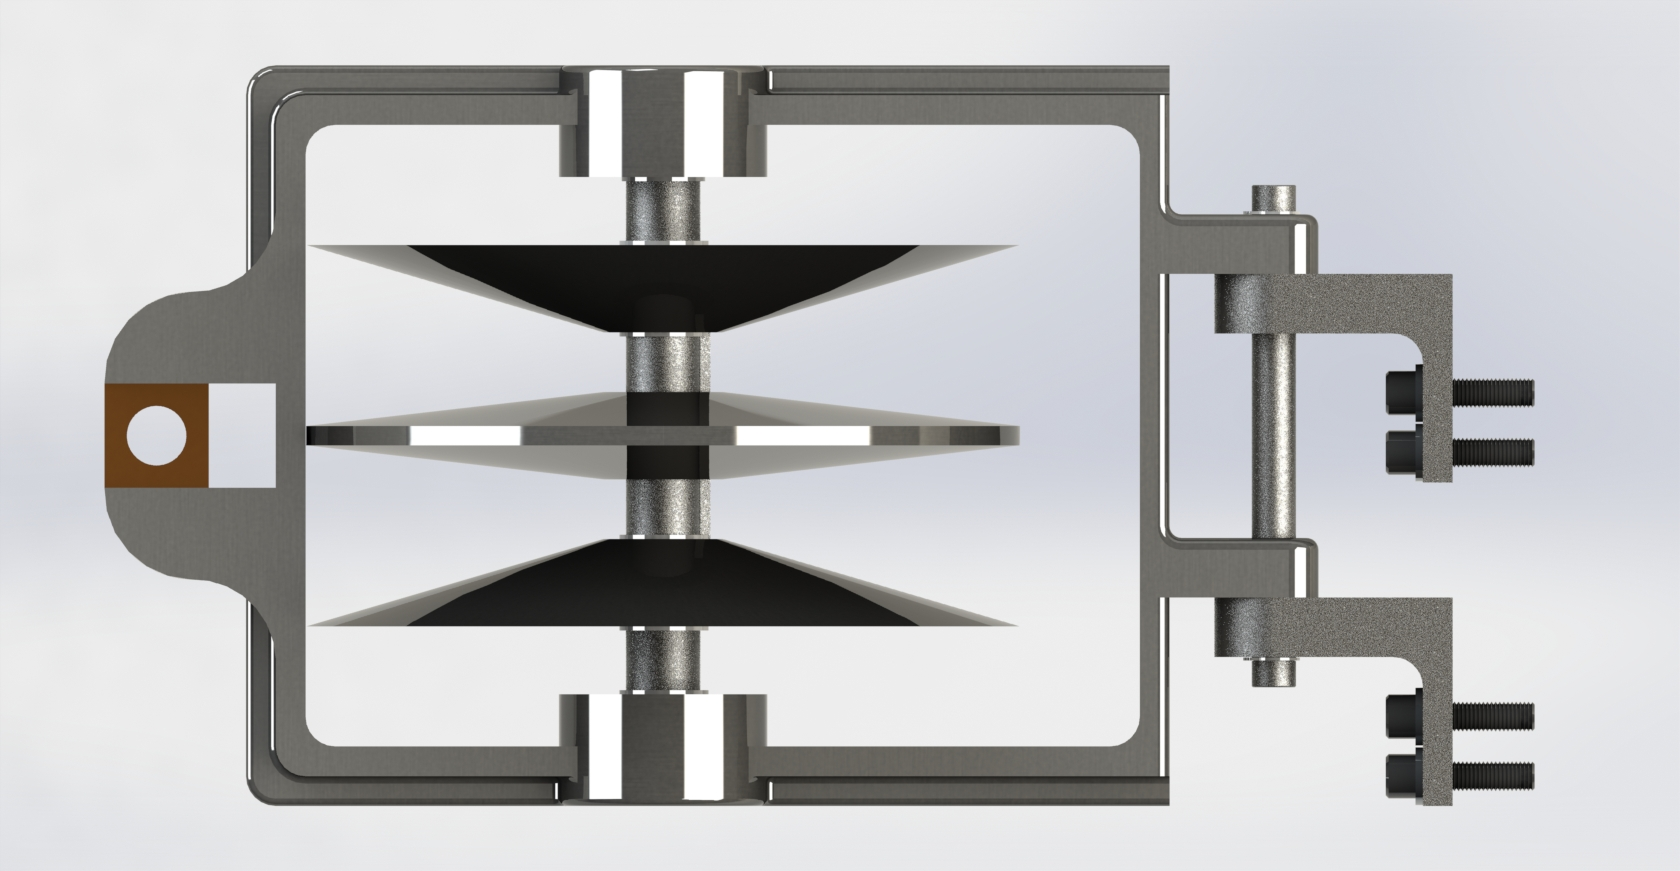
\includegraphics[width=0.6\textwidth]{./fall-report pictures/Chapter2-MachineDescription/VFC}
    \caption{SolidWorks rendering of the variator frame countershaft without belts}
    \label{fig:VFC}
\end{figure}

In order to maintain dynamic stability within this system, the variator frame is adjusted by way of a DC servomotor, a 10:1 reducing gearbox, and a 1/5” pitch multistart precision ACME feed screw. Although the components within this portion of the variator subassembly were selected primarily due to the availability of the parts, the 10:1 gearbox not only allows for finer grained control of the variator position, but also increases the effective holding torque of the feedscrew. 

\begin{figure}[H]
    \centering
    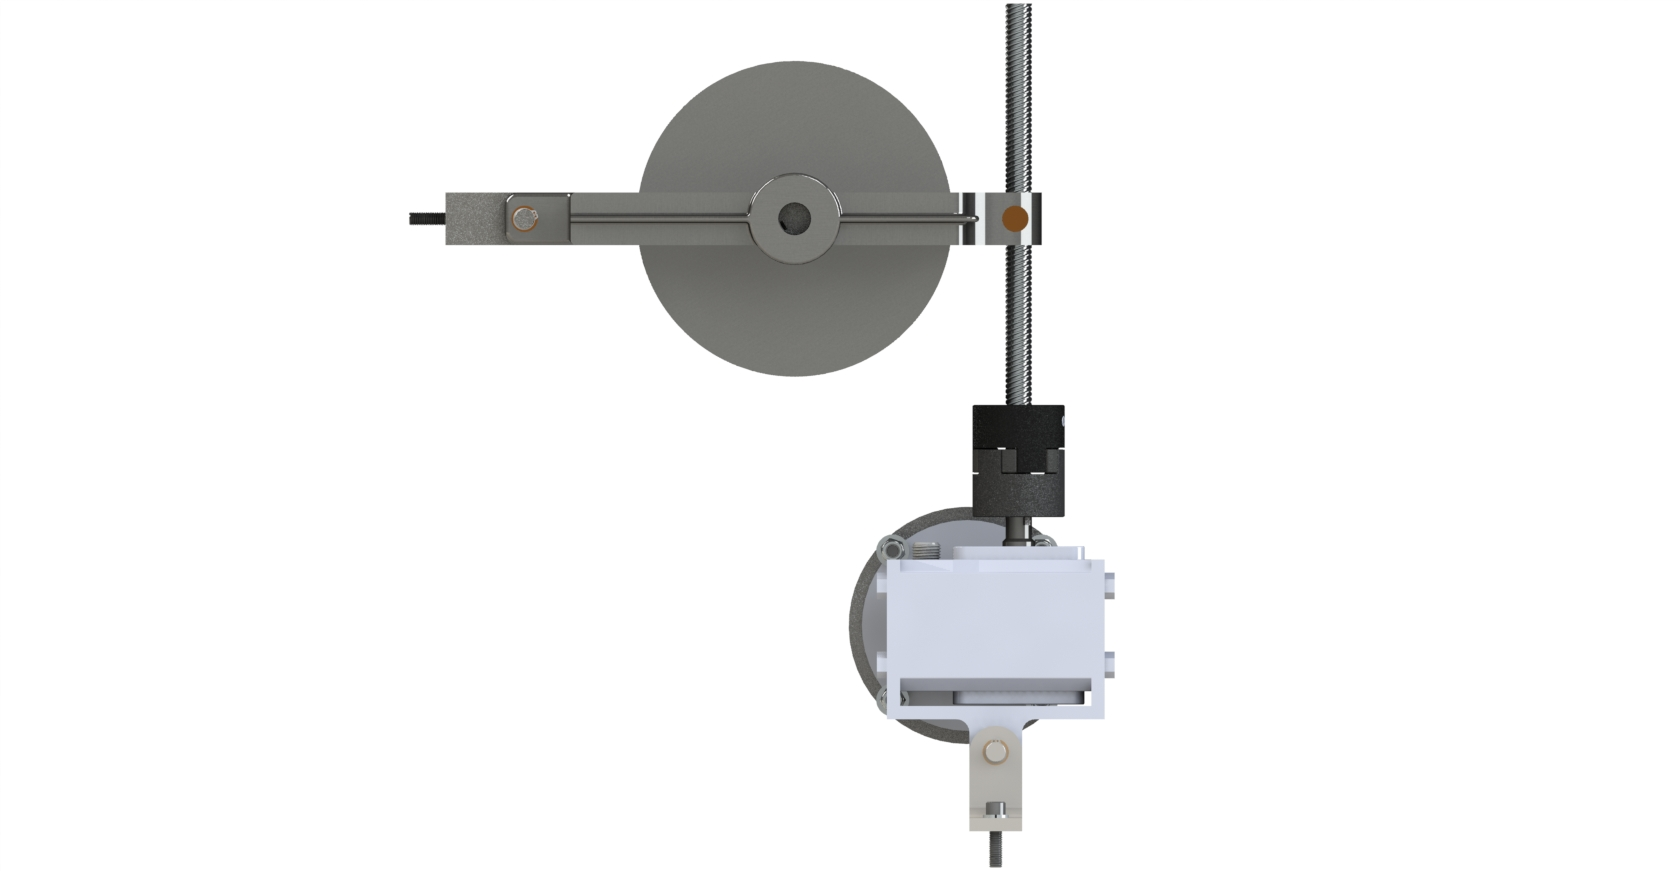
\includegraphics[width=0.6\textwidth]{./fall-report pictures/Chapter2-MachineDescription/DCGF}
    \caption{SolidWorks rendering of the DC motor, gearbox, and feedscrew}
    \label{fig:DCGF}
\end{figure}

On the opposite side of the variator’s countershaft is the upper variable speed belt which runs to the top-end variable speed pulley. This pulley is identical to the bottom end pulley except for the bore diameter. On this top pulley, the bore diameter is 3/8” larger than on the bottom pulley. This top pulley is keyed to the rear headstock driveshaft. The rear headstock driveshaft serves as the fixed reference point for the entire headstock driveshaft assembly. At the termination of the rear driveshaft is a press-fit CV-joint housing. This press fit, rated to three times the full-load stall torque transmits the rotational power to the mid-shaft. The mid-shaft terminates in a second CV-joint which is keyed to the spindle nose. The decision to use a key rather than a press fit was motivated the requirement that the spindle bearings be lubricated after every 50 hours of service. 

\begin{figure}[H]
    \centering
    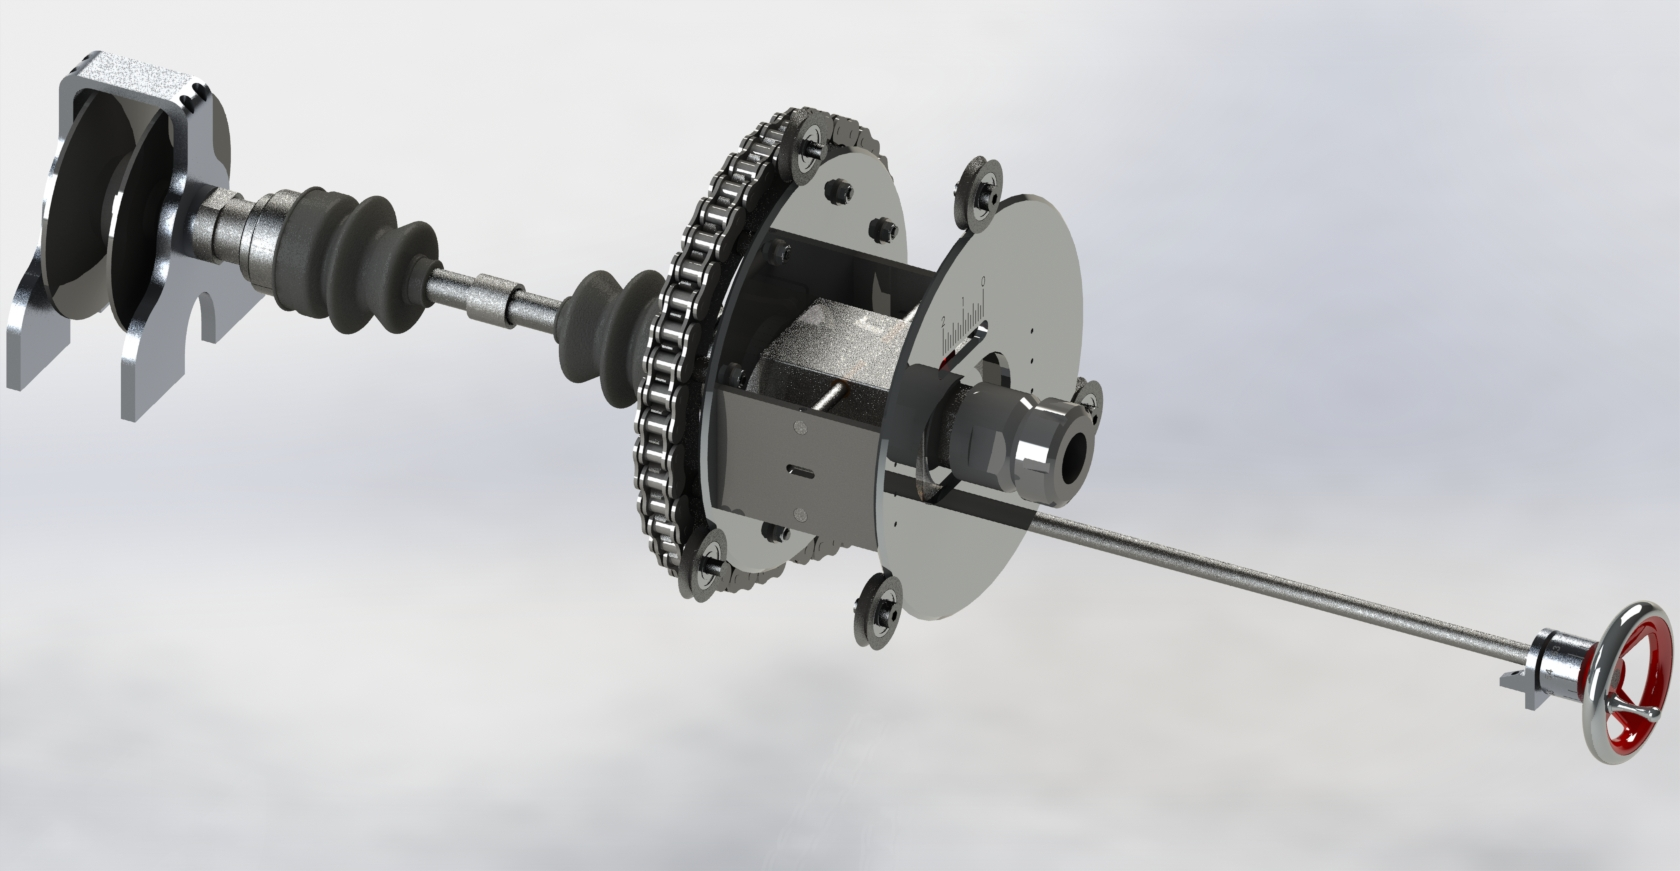
\includegraphics[width=0.6\textwidth]{./fall-report pictures/Chapter2-MachineDescription/HD}
    \caption{SolidWorks rendering of the overall headstock driveshaft assemblies}
    \label{fig:HD}
\end{figure}

The spindle nose eccentric mechanism is where the Notchmatic differs from the others on the market. The spindle bearings are embedded within a bearing block which slides along a pair of precision ground 1045 steel rods. The position of this bearing block is driven by a 1/2-10 ACME threaded rod which enters from the side of the eccentric mechanism. In order to increase the effective stiffness of the system, a pair of precision ground carrier plates form the guide ways along which the bearing block travels. The whole eccentric mechanism is driven by No. 60H ANSI roller chain. This roller chain variant is capable of withstanding upwards of 2000 lbf in normal operation. The 1:5 drive sprocket ratio ensures that the operator will not have to exert much force in order to notch thick-walled tubing. 

\begin{figure}[H]
    \centering
    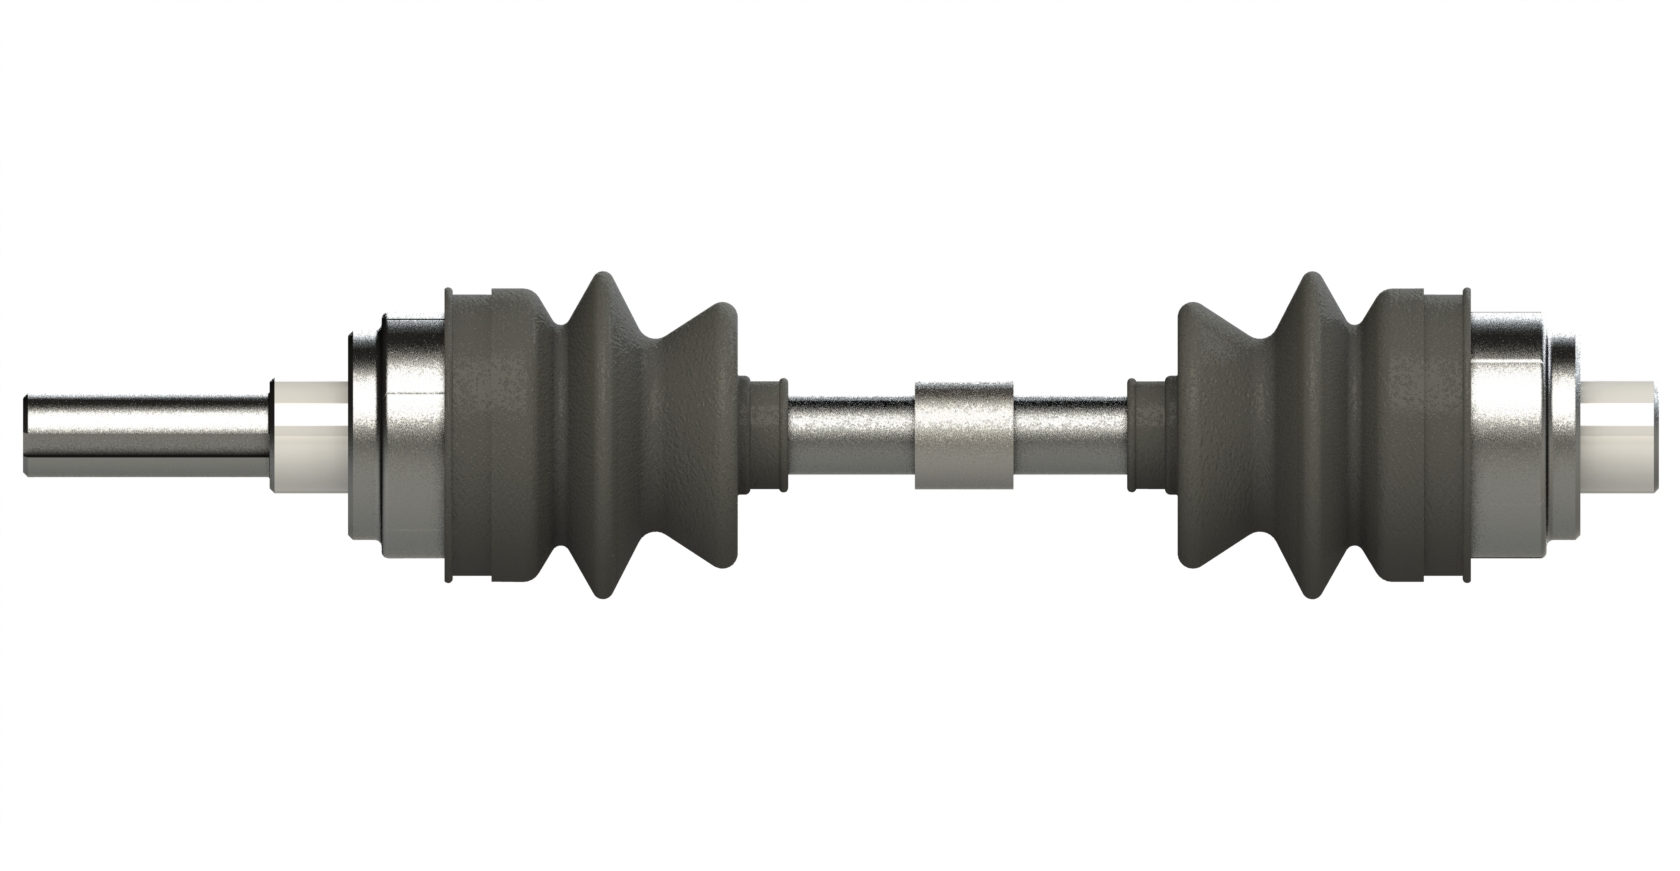
\includegraphics[width=0.6\textwidth]{./fall-report pictures/Chapter2-MachineDescription/Eccentric}
    \caption{SolidWorks rendering of the Eccentric Assembly}
    \label{fig:Eccentric}
\end{figure}

Tool holding for the Notchmatic is achieved through the use of an ER-40 collet holder. This allows greater flexibility of the selected tool. The recommended cutting tool for the Notchmatic is a 1” nitride coated roughing end mill. This style of tool pairs well with the Notchmatic’s wide speed range.

%-------------------------------------------------------------------------------------------------------------------------------------------------------------------------------------------------------------------------------------------------------------------------------------------------------------------------------------------------------------------------------------------------------------------------------------------------------------------------
\newpage

\subsection{Fixturing}

\begin{figure}[H]
    \centering
    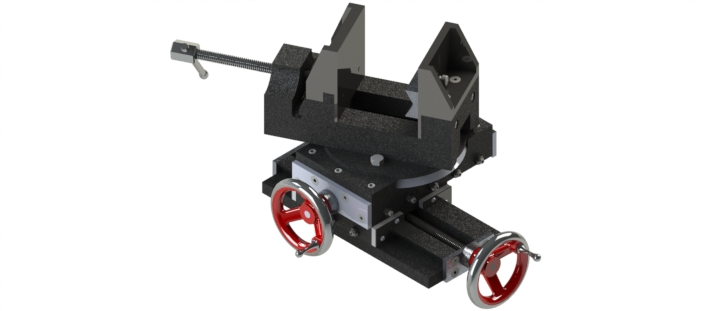
\includegraphics[width=0.6\textwidth]{./fall-report pictures/Chapter2-MachineDescription/Fixturing}
    \caption{SolidWorks rendering of the Full Fixturing Mechanism}
    \label{fig:Electrical:Fixturing}
\end{figure}

The fixturing mechanism for the Notchmatic assembly allows the workpiece to be positioned using three translational and one rotational degree of freedom. This allows the user to position the tube for centered notches, offset notches, angled notches, and even plunge cuts. Plunge cuts, however, require the user to purchase and use a separate end mills than the one currently used in the design. The full fixturing mechanism, shown above, is made from three main components; the dovetail slides, the rotational plate, and the vice. In the design of these components, it is critical that all loading conditions were considered. Thus, the material and fixturing decisions were made contingent upon the force analysis and calculations. 

The dovetail slides, shown below, make up a large portion of the fixturing mechanism. The slides allow the workpiece to be moved horizontally along the machine table. The bottom "x" direction dovetail slide is mounted to the steel bed in the structure of the Notchmatic. This bottom dove tail slide uses a lead screw to move the top dovetail slide and consequently the rest of the fixturing apparatus. The dovetails slides will be machined from cast iron bars and will be fitted with cutom made lead screws. To operate the dovetail slides and position the workpiece, handwheels rotate the leadscrews resulting in translational movement. The image below shows a top view of the dovetail slide and its placement on the structure of the machine. 

\begin{figure}[H]
    \centering
    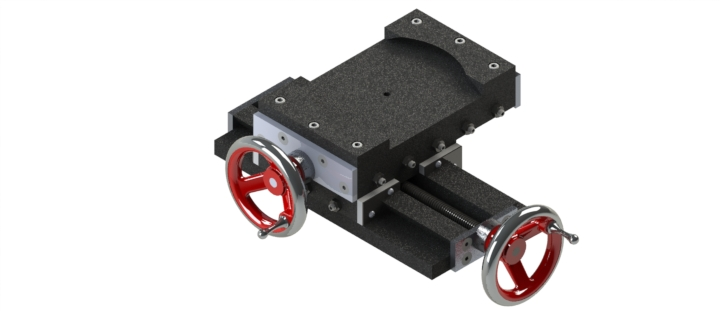
\includegraphics[width=0.6\textwidth]{./fall-report pictures/Chapter2-MachineDescription/Slide}
    \caption{SolidWorks rendering of the Slide}
    \label{fig:Electrical:Slide}
\end{figure}

\begin{figure}[H]
    \centering
    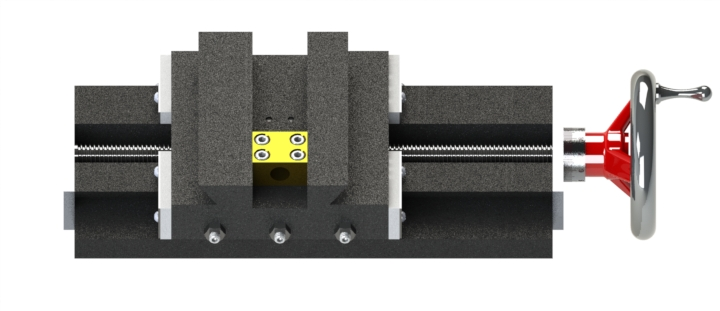
\includegraphics[width=0.6\textwidth]{./fall-report pictures/Chapter2-MachineDescription/Slide2}
    \caption{SolidWorks rendering of the Slide}
    \label{fig:Electrical:Slide}
\end{figure}

On top of the slides is the rotational plate. The rotational plate provides the rotational degree of freedom so that angled cuts can be made into the workpiece. The rotation requires two plates; a pressure plate and a swivel plate. Both plates will be machined in house from raw materials. The block is rotated by lifting a cam handle and manually rotating the plate before locking the piece. To clamp, two screws are tightened which allows the plate to clamp to the swivel blocks mounted on the top of the dovetail stage. Like the slides, the rotating mechanism is made from steel and will require regular lubrication to function properly. The top swivel plate holds the vice which houses the workpiece. The vice is a standard machining vice that uses a lead screw to secure the piece. Since the workpiece on the Notchmatic is likely to be rounded, a vice jaw extension attachment will be custom made and attached to the original jaw. The vise jaw extensions will be made from welded plates and will be screwed onto the original jaws. They are sized to comfortably hold the smallest to largest tube diameters; 1in to 3.5in, respectively. This jaw can be moved towards or away from the bed of the launcher giving the final vertical degree of freedom. A thumb screw is used to set the jaw in place. The tube fits snugly in the jaw because it includes a v-block. The rotational block, vice, and jaw components are shown in the figure below. 

\begin{figure}[H]
    \centering
    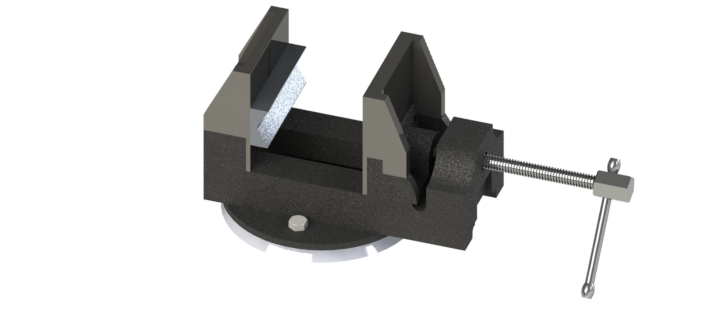
\includegraphics[width=0.6\textwidth]{./fall-report pictures/Chapter2-MachineDescription/Vice}
    \caption{SolidWorks rendering of the Rotating Plates, Vice, and Jaw of the Fixturing Mechanism}
    \label{fig:Electrical:Vice}
\end{figure}

%--------------------------------------------------------------------------------------------------------------------------------------------------------------------------------------------------------------------------------------------------------------------------------------------------------------------------
\newpage

\subsection{Electrical}
The electrical system is broken into two main sections; the circuit design and the electrical components. The circuit design includes all of the wired connections and safety of the electrical system in addition to their placement on the overall design of the tube notcher. The switches were selected according to these needs and were considered in parallel to the circuit design.  
\subsubsection{Circuit Design}
The circuitry of the tube notcher is broken into the AC and DC power lines. The AC power line controls the spindle AC motor which drives the cutting tool. The DC power line, on the other hand, controls the variator motor driving the continuous variable transmission. The majority of the safety features are included in the DC Line. The circuit begins from the wall outlet which provides 120VAC single phase. After the outlet, the first component is an anti automatic restart protection plug. For safety reasons, this is a critical component in the circuit for the tube notcher. After the protection plug, there is a 20A circuit breaker. From here, the power line is split between AC line and the DC line, as described earlier. A schematic of the wall components is shown below. 

\begin{figure}[H]
    \centering
    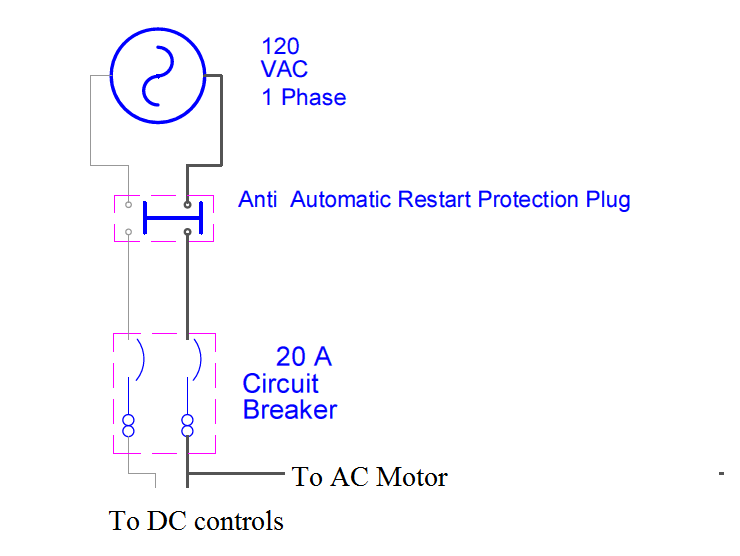
\includegraphics[width=0.6\textwidth]{./fall-report pictures/Chapter2-MachineDescription/Wall}
    \caption{Schematic of the wall outlet connections and components}
    \label{fig:Electrical:Wall}
\end{figure}

The AC line is the simpler of the two lines and is composed of only 2 components. First, there is a drum switch that controls the rotational direction, including netural, of the spindle. The spindle is driven by an AC motor. The entire AC line is shown in the figure below. The additional on/off control of the motor, however, is controlled by relays which are included in the DC line.

\begin{figure}[H]
    \centering
    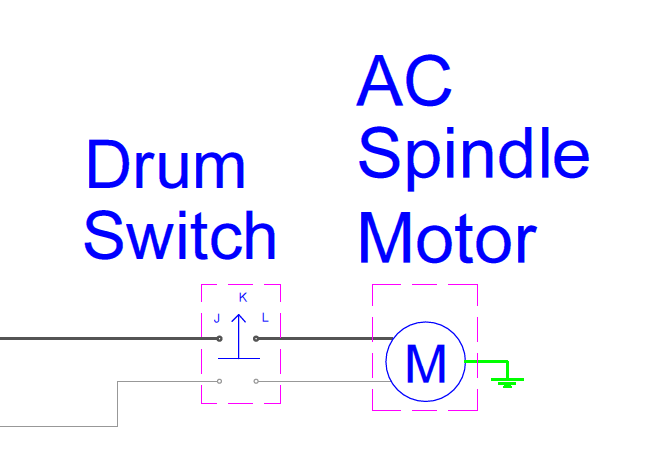
\includegraphics[width=0.6\textwidth]{./fall-report pictures/Chapter2-MachineDescription/AC}
    \caption{Schematic of the AC line}
    \label{fig:Electrical:AC}
\end{figure} 

The DC line includes the majority of the circuitry for the tube notcher. Because the power originally starts from the wall, the first step in the DC line is to convert the voltage from 120VAC to 12VDC. This is done in two stages. First, a transformer steps down the voltage from 120 VAC to 12 VAC. Then, a full wave rectifier converts the 12VAC into 12VDC. To protect the rest of the circuit, a 20A fuse is connected at the output of the positive DC terminal of the full wave rectifier. Capacitors are connected from the DC positive to DC negative in order to smooth out the DC output from the rectifier. This will provide power and ground the DC controls. This segment of the DC circuit is shown in the following figure.

\begin{figure}[H]
    \centering
    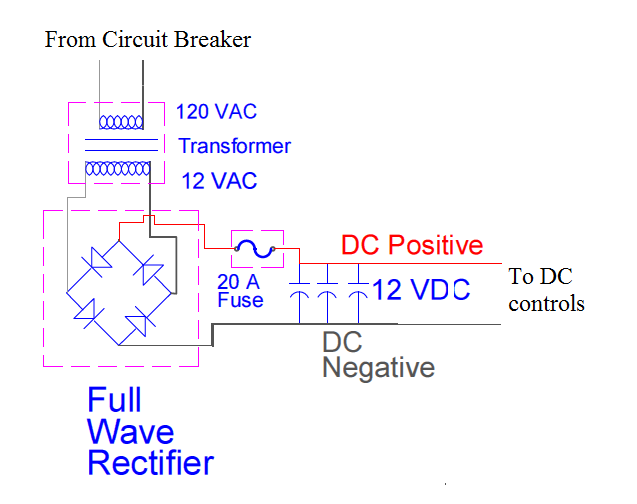
\includegraphics[width=0.6\textwidth]{./fall-report pictures/Chapter2-MachineDescription/ACDC}
    \caption{Schematic of the AC to DC conversion}
    \label{fig:Electrical:AC}
\end{figure} 

\newpage
The remainder of the DC line includes the switches and relays that allow the tube notcher to function. Also included are the safety features which will be elaborated on in the following section. In total, there are 7 switches and 6 relays.

\begin{figure}[H]
    \centering
    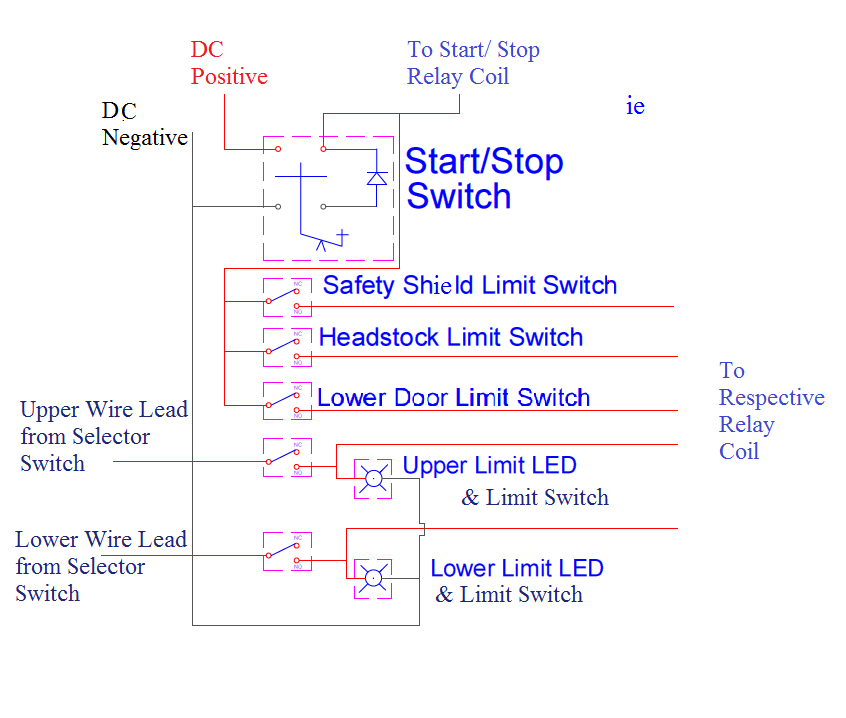
\includegraphics[width=0.6\textwidth]{./fall-report pictures/Chapter2-MachineDescription/Switches}
    \caption{Schematic of the Start/Stop and Limit Switches}
    \label{fig:Electrical:Switches}
\end{figure} 

The figure above depicts 6 of the switches used in the tube notchers design; the start/stop, safety shield, headstock, lower door, and variator limit switches. DC positive and negative lines are connected to the terminals of the start/ stop switch. Once the start/ stop switch is turned ``on'', all the limit switches have a source of power, except the upper and lower limit switch which are powered by the selector switch. The start/ stop is connected to a relay coil which will turn on the AC and DC motors of the tube notcher. It is very important that the DC motor only runs when the AC motor is also running. If DC motor runs when the AC motor is ”off”, the belts of the variator pulley will experience slack, become loose and belt will slip off the pulley.

There are various limit switches on the tube notcher that mainly control corresponding relays to turn the AC and DC motors ``off'' or ``on''. All the limit switches are Ormon Z-15GW2-B, which has a long lever arm with a wheel at the end. The limit switches are connected to a relay coil which will turn ``on/off'' the AC and DC motors of the tube notcher. When the limit switch contacts are close, the relay coils are magnetize. All of the limit switches are placed in series with one another. 

The safety shield limit switch contact is closed when the safety shield is covering the cutting tool and  pushing the lever arm of the limit switch. Similiarly, the headstock door and lower door limit switches contacts are closed when the door closes and pushes the lever arm of the limit switch. The last two limit switches are for the variator pulleys. It is critical that the variator pulleys do not over-travel beyond the upper and lower limits. Therefore, there are limit switches for the upper and lower limits of the variator pulley. When the pulley contacts the  lever arm, the limit switch contact is close, providing power the relay coil to turn the DC motor off.

The final switch is the 3-position center-return selector switch; depicted below. The 3 position selector switch is used for controlling the vertical position of the variator pulley by driving a DC motor that is attached to a feed screw that vertically positions the variator pulley. The selector switch has 3 positions: ``increase''(left position), ``stop'' (center position), and ``decrease'' (right position). At the center position, all the contacts of selector switch are open which doesn’t provide power to the DC motor, hence this is the ”stop” position. When the knob is at the ”increase” position (left position), the upper two contacts are closed and the bottom two contacts are opened, as seen below. The top wire lead is positive and the lower lead is negative which causes the DC motor to spin in a direction that moves the variator pulley upwards. In the ”decrease” position (right position), the upper two contacts are opened and the bottom two contacts are closed which changes the polarity of the DC motor. Opposite of the ”increase” position, the polarity of the DC motor wire lead is reverse: the top wire lead is negative and the lower lead is positive which causes the DC motor to spin a direction that moves the variator pulley downwards. When the top wire lead is positive (``increase'' position ) , power is provide for the upper limit switch. With power, when variator pulley over-travels, the upper limit switch is able to magnetize the relay coil to turn the DC motor off. This is equivalent to a ``AND'' logic; when ``increase'' position is selected AND upper limit switch is pushed, then the DC motor can turn off.  The red ``increase'' LED indicator turns to indict over-traveling. When the user selects the ``decrease'' position, the DC motor regains power.

\begin{figure}[H]
    \centering
    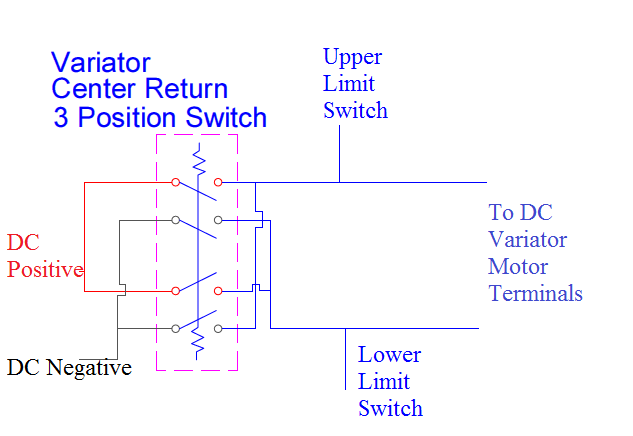
\includegraphics[width=0.6\textwidth]{./fall-report pictures/Chapter2-MachineDescription/3PSwitch}
    \caption{Schematic of the 3-position center-return selector switch}
    \label{fig:Electrical:3PSwitch}
\end{figure} 

Relays are used for controlling on/off for both AC and DC motors of the tube notcher. There is an emergency button that opens the contacts for both motors when the button is press. The relay are DPDT which means double pole double throw. Below is a schematic of a DPDT start/stop relay. Double poles means there are two separate contacts that are triggered by magnetized coil. Double throw means for each contact, there is a normally closed terminal (NC) and a normally opened terminal (NO) that shared a common terminal (left side of the contacts). When the coil is not magnetized, the contact is unmoved causing the common terminal and normally closed terminal to be connected. When the coil is magnetized by a limit switch or start/stop button providing current into the coil, the contact is shifted causing the common terminal and normally opened terminal to be connected. There is a flyback diode connected in parallel with the coil to prevent high current spikes when the contact that provides current to the coil is closed.
\begin{figure}[H]
    \centering
    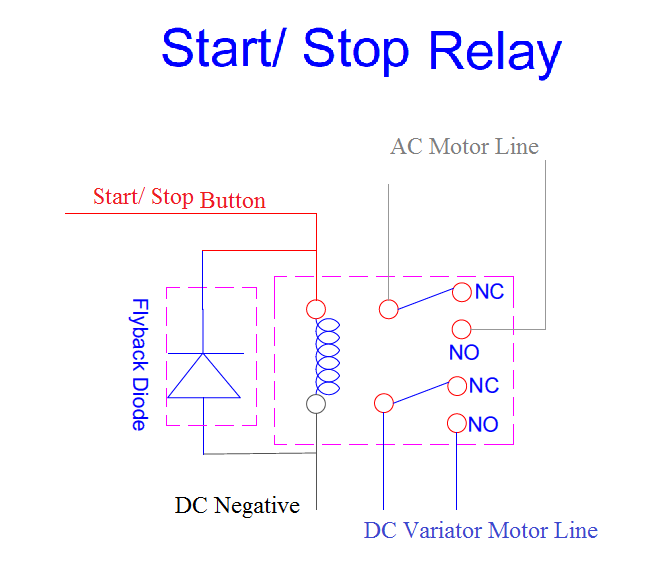
\includegraphics[width=0.6\textwidth]{./fall-report pictures/Chapter2-MachineDescription/RelayPic}
    \caption{Schematic of the Start/Stop Switch Relay}
    \label{fig:Electrical:StartStopSwitchRelay}
\end{figure} 

The relay contacts and emergency button are connected in series. This is equivalent to an OR logic which means the motors will turn off when any of the limit switches, emergency button or start/stop button is triggered. This a safety feature of the tube notcher. 
The normally opened terminals of the start/stop relay, safely shield relay, headstock relay and lower door relay are connected in series for each motor connection and their contacts will closed  when their respective limit switch or start/stop button provides current. 
For the DC motor, in addition to those relays, the normally closed terminals of the upper variator relay and lower variator relay are also connected in series. Their contacts will open when their respective limit switch is closed by the variator pulley pushing the lever arm.
In this relay connection, the case, as mentioned before, when the AC motor is off and the DC motor is on cannot happen. 
\begin{figure}[H]
    \centering
    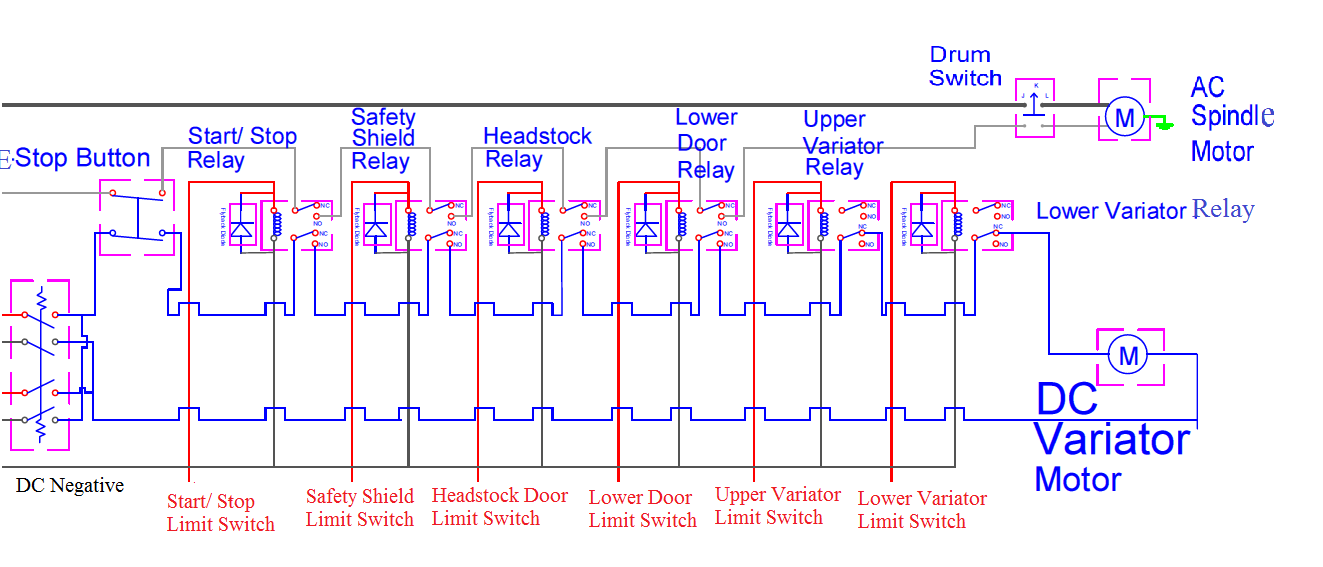
\includegraphics[width=0.6\textwidth]{./fall-report pictures/Chapter2-MachineDescription/Relays}
    \caption{Schematic of the Relays}
    \label{fig:Electrical:Relays}
\end{figure} 

\subsubsection{Electrical Components}
The control aspects of the tube notcher are kept under low voltage DC. Keeping a lower voltage is safer for the user and cost efficient. To simplify maintence and part replacement only one type of relay and limit switch is used in the design. The relay and socket come inpairs. The particular relay used in Notchmatic's design has a good reputation in industry for being reliable and robust. Although, the power rating for this relay is beyond what the tube notcher is expected to experience, these relays are not as expensive as other relays of similar performance. These relays are also popular in industry; making replacement for these relays less difficult. This relay is DPDT which means it provides normally opened and closed connections while other relays provide only normally opened or normally closed for the same cost. Additionally, socket mounts provides modularity, meaning relays can be swap and if a relay fails, the socket will not need to be replace. The screw terminals provide easier wire connections.

Like the relays, the limit switches on the Notchmatic have a good reputation in industry. They have a long lever arm that is more rigid than other limit switches. The mechanical life is expected to be over 5 million cycles and the electrical life is expected to be over 1 million cycles. The switches have holes for mounting and are easily wired using screw terminals.

As described earlier, an anti-restart plug is included into the design. According to OSHA safety standards, small motor machines must have an anti restart device to prevent the machine from restarting when there is a power interruption. This anti restart plug is easily attached to the tube notcher before connected to the outlet.

\newpage
\begin{figure}[H]
    \centering
    
\includegraphics[width=0.6\textwidth]{./fall-report pictures/Chapter2-MachineDescription/ControlBox}
    \caption{Solidworks rendering of of the Control Box}
    \label{fig:Control Boxl}
\end{figure} 

The majority of the electrical system's components are placed in three locations, the control box, the control panel, and the safety shield. The control box is located at the bottom of the Notchmatic, as shown in the figure above. It contains the relays and other circuit components that are included in the design. The majority of the switches, however, are located on the control panel. The control panel as seen below, is mounted to the headstock and has the majority of the switches that operate the machine. The switches that are not on the control panel are the limit switches. These are located on the safety shield, see below, and on the variator pully ends. Access to all the switches were made easy so that even an amateur macinist could operate the Notchmatic with ease. 

\begin{figure}[htp]
    \centering
    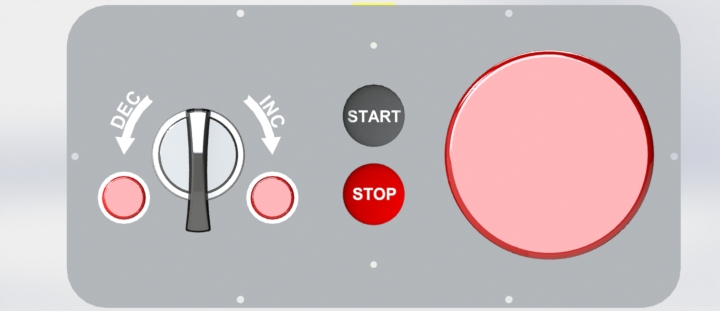
\includegraphics[width=0.6\textwidth]{./fall-report pictures/Chapter2-MachineDescription/ControlPanel}
    \caption{SolidWorks rendering of the Control Panel}
    \label{fig:Control Panel}
\end{figure}
 
\begin{figure}[hbp]
    \centering
    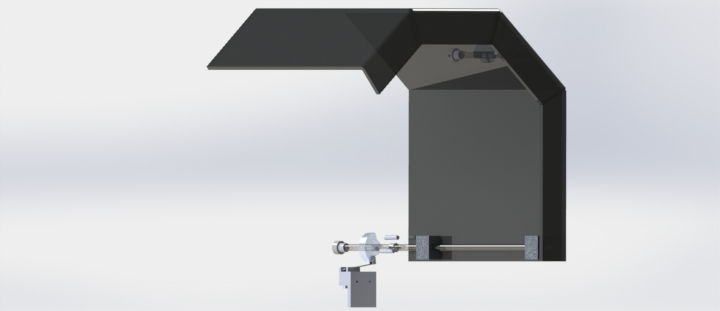
\includegraphics[width=0.6\textwidth]{./fall-report pictures/Chapter2-MachineDescription/Shield}
    \caption{SolidWorks rendering of the Safety Shield}
    \label{fig:Control Panel}
\end{figure} 